\section[q3]{Question 3}
\textit{Is there an association between year [as a continuous variable, use all years to perform
the analysis] and pm25\_concentration.}

\subsection{Question 3.a}
\textit{Plot a single graph/figure showing the relationship between these two variables.}

\begin{figure}[H]
    \centering
    % 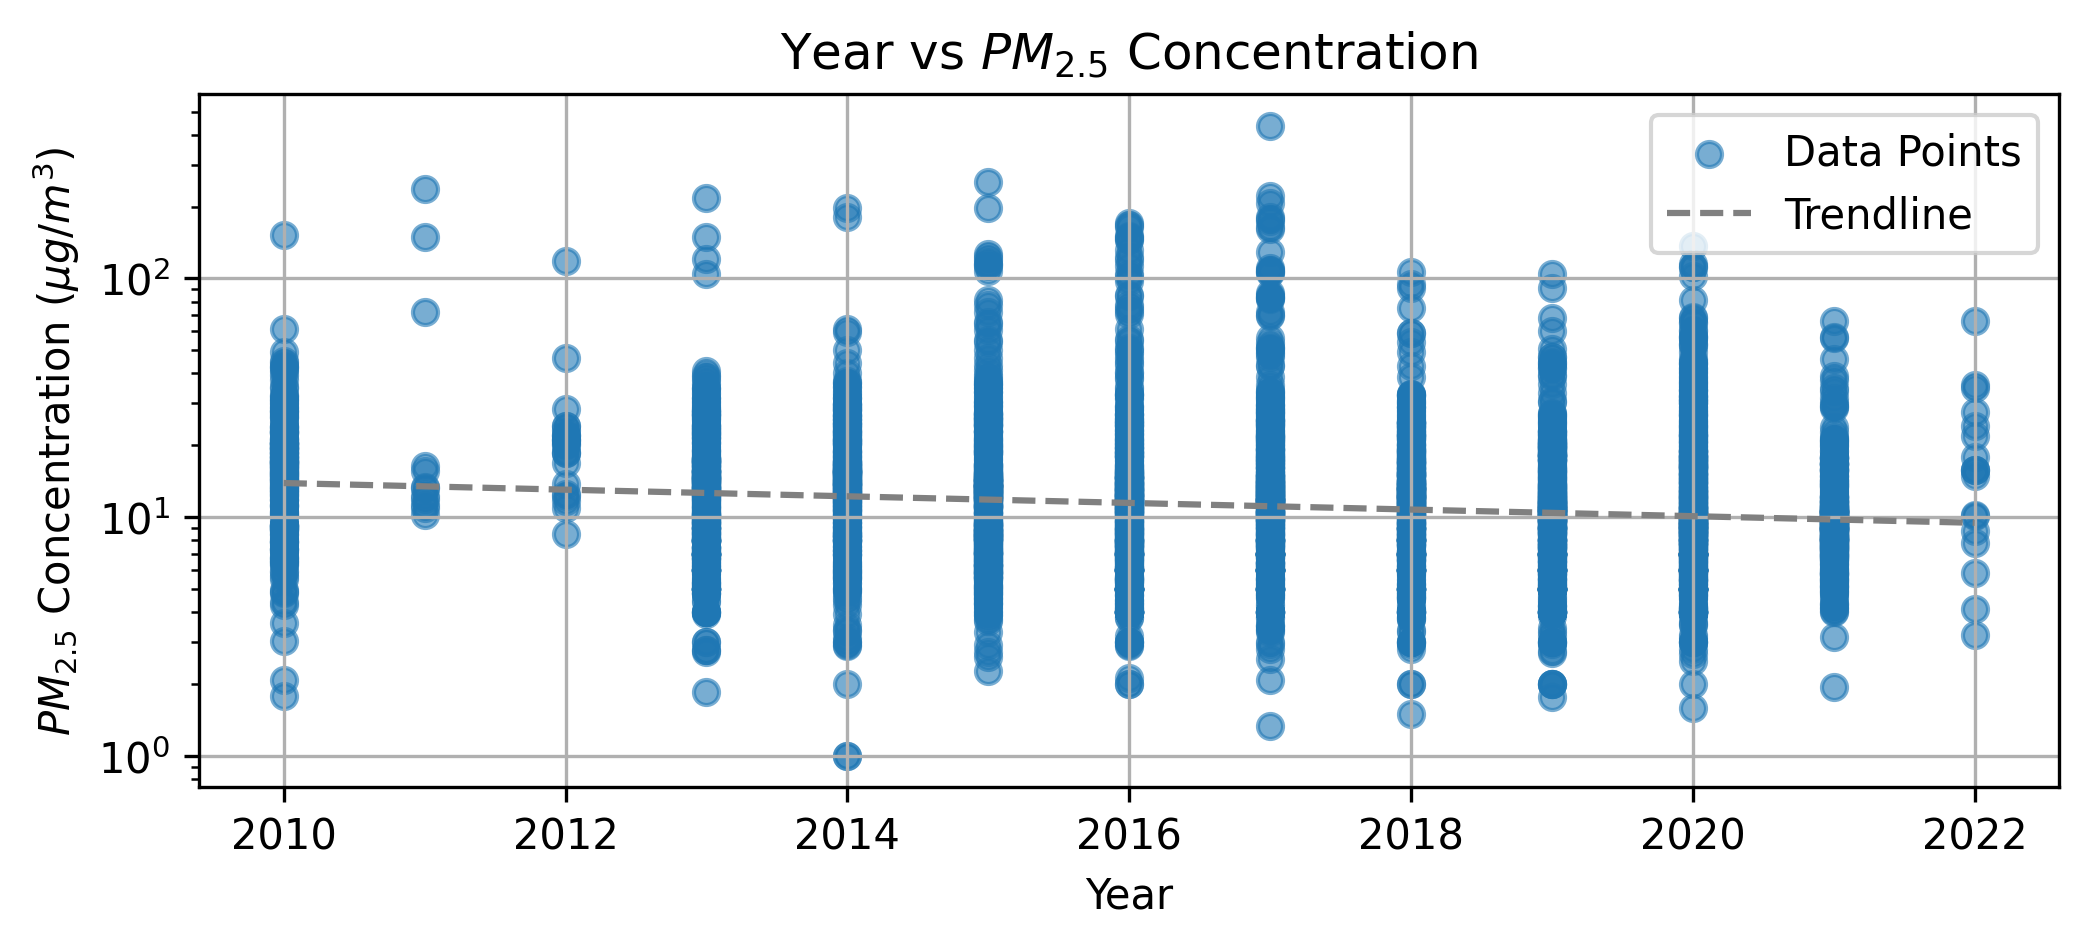
\includegraphics[width=\textwidth]{img/q3_year_vs_pm25log.png}
    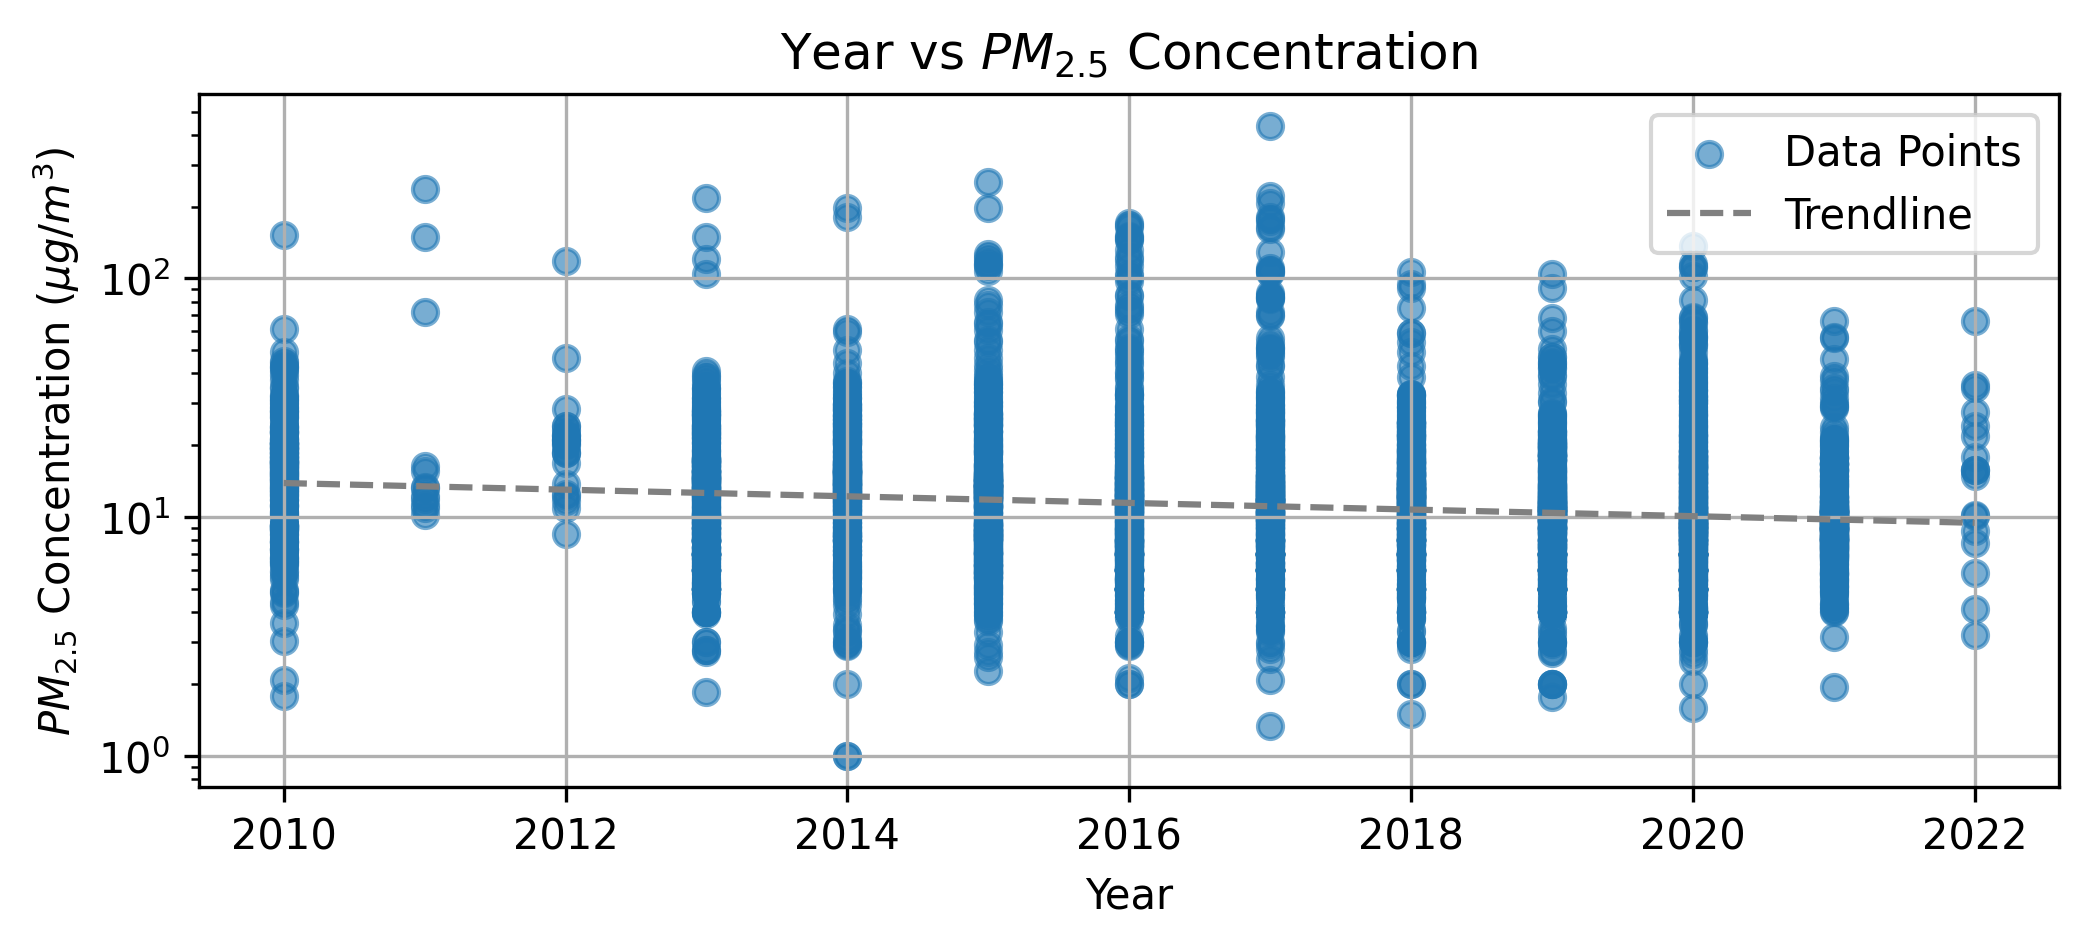
\includegraphics[width=0.8\textwidth]{img/q3_year_vs_pm25log.png}
    \caption{Relationship between year and $PM_{2.5}$ concentration.}
    \label{fig:year_pm25_relationship}
\end{figure}


\subsection{Question 3.b}
\textit{Select an appropriate statistical test for correlation.
Check the assumptions of your chosen statistical test for correlation. Report
your decisions on the validity of the assumptions for your chosen statistical test. Justify your decisions.
Report the name of the final test you choose to run}

\paragraph*{Step 1: Check for normality}
Year is ordinal data. Although it is used as contnuous data for the correlation test, it will not be normall distributed.  Normality of To determine of $PM_{2.5}$ concentration has already been tested in question 2 using the Shapiro-Wilk test.

\begin{itemize}
    \item $H_0$: $PM_{2.5}$ concentration is normally distributed.
    \item $H_A$: $PM_{2.5}$ concentration is not normally distributed.
\end{itemize}

The $p$-value of the Shapiro-Wilk test is $< 0.05$. Thus, we reject $H_0$ and conclude that the data is not normally distributed.

\paragraph*{Step 2: Check for monotonicity}
The scatterplot in Figure \ref{fig:year_pm25_relationship} shows a negative correlation between year and $PM_{2.5}$ concentration. The data points appear to follow a general downward trend and suggests that the relationship is monotonic.

Since neither variable is normally distributed and the data is monotonic, the Spearman rank correlation coefficient is used to determine a correlation coefficient.


\subsection{Question 3.c}
\textit{Run your chosen test, report the p-value and report on the magnitude and
direction of the effect (use the test results and refer to your figure from 3a).}

The Spearman rank correlation coefficient is used to determine the correlation between year and $PM_{2.5}$ concentration. The code used to determine the Spearman rank correlation are shown in Listing \ref{lst:pm25year}.
The Spearman rank correlation coefficient is $-0.163$, indicating a weak negative correlation between year and $PM_{2.5}$ concentration. The $p$-value is $< 0.05$, indicating a that there is a monotonic relationship between year and $PM_{2.5}$ concentration that is not by chance. This slight negative slant can be seen by the grey line in Figure \ref{fig:year_pm25_relationship}.\\

\begin{lstlisting}[caption={Python code to evaluate correlation between $PM_{2.5}$ concentration and year}, label={lst:pm25year}]
    spearman_corr, spearman_pval = spearmanr(years, pm25)

    print(f"Spearman's correlation: {spearman_corr}")
    print(f"P-value: {spearman_pval}")
\end{lstlisting}

\newpage